\documentclass[letterpaper, 11 pt, conference]{IEEEtran}

\usepackage{flushend}
\usepackage{graphicx}
\usepackage{listings}
\lstdefinestyle{mystyle}{
	basicstyle=\footnotesize,
	breakatwhitespace=false,         
	breaklines=true,                 
	captionpos=b,                    
	keepspaces=true,                 
	numbers=left,                    
	numbersep=5pt,       
	numberstyle=\tiny,           
	showspaces=false,                
	showstringspaces=false,
	showtabs=false,            
	tabsize=2
}

\lstset{style=mystyle}



%opening
\title{RIO Checkpoint/Restart Functionality Integration with CODES: Report}
\author{Neil McGlohon}
\date{November 2017}


\begin{document}

\maketitle

\begin{abstract}
	This report is meant as an informal introduction to RIO, Rensselaer's Optimistic Simulation System's checkpointing and restart module. I will start with an introduction to what RIO is as well as a brief roundup of its API. I also document the changes made to the CODES source to incorporate serialization of LP state. Finally I touch on the limitations of current RIO implementation and what is left for the future.
\end{abstract}

\section{Introduction}
An inevitable property of state-of-the-art research today is that it pushes against the boundaries of what was possible yesterday. Trends in HPC research are looking to design and simulate the best supercomputers of the future. To simulate larger and more complex supercomputer designs, we will need larger and more complex simulations. One caveat of larger-scale simulations is often increased simulation runtimes. As long as a simulation is running it is vulnerable to errors caused by the OS or the machine itself. It is vulnerable to time limits imposed on it by the system administrator. The longer the simulation runs, the more likely it is to run into such an issue. The workaround for these problems is to checkpoint a simulation so that it can be restarted from that checkpoint without losing any validity or determinism that was expected from an uninterrupted run. RIO, short for ROSS-Input/Output, is this workaround.


\subsection{What RIO is}
RIO is a checkpointing API for Rensselaer's Optimistic Simulation System (ROSS) developed by Elsa Gonsiorowski. It gives ROSS model developers the ability to save the entire simulation state so that it can be restarted from that saved point. Silently integrated into ROSS, it is inactive by default during the ROSS build process. It's designed so that no RIO code is reached unless it is turned on by the developer. 

In addition to changing a flag during building, the developer must also implement the necessary functions to serialize/deserialize model actors (LPs). RIO will wait until the scheduled end of the simulation and use the developer-implemented functions to serialize LP state to a buffer and use MPI-IO to write that buffer, in partitions, to multiple files in parallel. LP state is not the only important part of the simulation necessary to restart, however. There are likely events that were scheduled for after the planned end-time of the simulation waiting in event buffers - never to be delivered. If a restart is initiated and those events aren't present in those buffers, the simulation will not have the same validity or determinism as it did at the time of checkpointing. RIO captures those leftover events prior to ROSS finalizing cleanup and includes them in the checkpoint, loading them into the proper event buffers upon restart. This leaves the simulation state upon restart to be equivalent to that when it was checkpointed, therefore maintaining validity and determinism. 


\subsection{What RIO isn't}
RIO was not designed to be used directly for fault tolerance. That is, it was not designed for periodic checkpointing during the runtime of the simulation in preparation of unexpected errors. Doing so, while theoretically possible, would incur a large amount of time and space complexity to the execution of simulations. RIO saves events that were scheduled for after the end of the simulation. This happens at the \emph{planned} end time of the simulation, when all LPs agree on what time it currently is. It is the only time, apart from the beginning, where this is guaranteed to be the case. 

Because of the time-consensus between all actors in the simulation, there is no need to capture events that are saved in other event buffers: like the buffer that stores events that occurred after the latest GVT timestamp. If mid-simulation checkpointing was a part of RIO, it would have to save a lot more events, greatly increasing the disk space required to serialize all of the simulation. Additionally, checkpointing requires what is called a consistent cut of the simulation: something that may be possibly achieved during GVT all-to-all communication points. But while possible, larger simulations may experience increased slowdown due to all-to-all communication and barriers waiting for serialization to be completed. These challenges will be discussed at greater length in Section \ref{sec:challenge}.

\section{RIO API}
RIO was designed to work with ROSS and ROSS models when implemented by the model developers. One important feature of RIO is that it will work perfectly fine with dynamically allocated LP state. That being said, this feature requires more work to be put on the developer as it is impossible for RIO to know \emph{a priori} how much space is required to serialize LP state. Let alone even know where parts of the LP state are located as theres no guarantee of contiguous memory allocation between two different structures.

To get a ROSS model to work with RIO, there needs to be three functions implemented for each LP type in the simulation: 

\begin{itemize}
	\item Serialize
	\item Deserialize
	\item Size
\end{itemize}

The serialize and deserialize functions have a pointer to the LP state, a pointer to a valid buffer, and a pointer to the ROSS LP as parameters. They return nothing. The size method has the same parameters, excluding the buffer, and expects to return the size of the LP in question.

RIO expects that after the serialize function has been called in the checkpointing process, the buffer that was passed to it is filled with LP state in a model-developer-known schema. This same buffer will be passed to the deserialize function upon restart.

\subsection{CODES Specific RIO Changes}
CODES doesn't follow the ROSS way of LP type mapping and organization. Specifically, it doesn't use \texttt{g\_tw\_lp\_types} and related global values. RIO requires these in order to call the correct serialization functions when necessary. I've added some new features to RIO to allow for cleaner interfacing with ROSS than what was previously supported. 

This new API is designed to allow for LP types to be defined in different files and scopes - so long as each scope can still access the RIO library. This is the case for how CODES LP types are defined. RIO tutorials populate the necessary typemaps in the main method of the program. This same tactic won't work for CODES as LP types are defined in many different files and scopes - e.g. the main method can't see a simplenet or dragonfly router LP type and thus can't tell RIO about them. Those network models must each use the new API to tell RIO about their unique defined LP types.

The additions to RIO overcome this issue by creating a register visible by all of the RIO library and thus LP types can be passed into RIO from multiple locations in the CODES source. 

\section{Integrating RIO into a CODES Model}
There are three main steps to get RIO working on a CODES model:

\begin{enumerate}
	\item Write 3 RIO functions for each LP type in a simulation \label{step1}
	\item Inform RIO about the various LP types and their associated serialization functions \label{step2}
	\item Configure high-level RIO checkpointing behavior in main method \label{step3}
\end{enumerate}

In a general CODES modelnet simulation there are two classifications of LPs: Modelnet and Non-Modelnet. Examples of modelnet LPs are Dragonfly router and Simplenet LPs. An example of a non-modelnet LP is the server LP types defined in synthetic workload sources.

\subsection{Step 1: Implementing the RIO API}

\subsubsection{Serializing Non-Modelnet LPs}
This is the most straight forward portion of RIO integration with a model. So long as the LP types are registered using the above mentioned functions and the three main RIO API methods are implemented, then RIO can easily serialize these types of LPs. An example of an LP that would be serialized this way would be workload related LPs: like the \texttt{svr\_lp} LP found in \texttt{modelnet-test.c}.

\subsubsection{Serializing Modelnet Base LP}
This is the first of proposed permanent changes to main CODES modelnet source. The modelnet base LP acts as a wrapper for any modelnet LP type (e.g. Dragonfly Router, Dragonfly Terminal, Simplenet LP, \ldots). It has its own state associated with it as well as pointers to the necessary sub-LP state. I've written the serialization functions for the modelnet base lp and added additional state to house the function pointer struct for the subtype RIO functions. This involved adding new methods to the CODES global `method array' in a similar way to how Caitlin Ross' ROSS instrumentation was integrated.

\subsubsection{Serializing Modelnet Network LPs}
This is the main portion of RIO integration with CODES that is left to the model developers themselves. The previously mentioned modelnet base LP serialization will be used in all CODES simulations but different simulations will have different network models. For example, Simplenet has a single LP type defined in it, Dragonfly has two and RIO functions must be implemented for each LP type used in the simulation. 


\subsubsection{Example: Simplenet LP Serialization Functions}
To serialize any LP will generally require more effort than a single \texttt{sizeof()} call paired with a \texttt{mempcpy()} command. The simplenet LP state is almost as simple as that if not for the dynamic character array, \texttt{anno}.

\begin{lstlisting}[language=C]
struct sn_state
{
	tw_stime net_send_next_idle;
	tw_stime net_recv_next_idle;
	const char * anno;
	simplenet_param params;
	struct mn_stats sn_stats_array[CATEGORY_MAX];
};
\end{lstlisting}

The process of serialization for this LP will be copying data that changes throughout the simulation into a preallocated buffer. Deserialization will be copying data from a supplied buffer back into the relevant state properties and re-initializing any other, simulation time-constant, properties.

\begin{lstlisting}[language=C]
static void sn_serialize(sn_state *s, void *buffer, tw_lp *lp) {
	size_t offset = 0;
	memcpy(buffer+offset, &s->net_send_next_idle, sizeof(tw_stime));
	offset+= sizeof(tw_stime);
	memcpy(buffer+offset, &s->net_recv_next_idle, sizeof(tw_stime));
	offset+= sizeof(tw_stime);
	memcpy(buffer+offset, &s->params, sizeof(simplenet_param));
	offset+= sizeof(simplenet_param);
	memcpy(buffer+offset, &s->sn_stats_array, sizeof(mn_stats)*CATEGORY_MAX);
	offset+= sizeof(mn_stats)*CATEGORY_MAX;
}
\end{lstlisting}

Looking at the serialization function, there's nothing particularly fancy in it. It simply copies the state into the supplied buffer. It is important, however, to note that the dynamic character array, \texttt{anno}, was not copied over. This character array doesn't change throughout the simulation so it wasn't important to save in a checkpoint - thus it wasn't serialized. We need to remember to re-initialize it upon deserialization.

\begin{lstlisting}[language=C]
static void sn_deserialize(sn_state *s, void * buffer, tw_lp *lp) {
	size_t offset = 0;
	memcpy(&s->net_send_next_idle, buffer+offset, sizeof(tw_stime));
	offset+= sizeof(tw_stime);
	memcpy(&s->net_recv_next_idle, buffer+offset, sizeof(tw_stime));
	offset+= sizeof(tw_stime);
	memcpy(&s->params, buffer+offset, sizeof(simplenet_param));
	offset+= sizeof(simplenet_param);
	memcpy(&s->sn_stats_array, buffer+offset, sizeof(mn_stats)*CATEGORY_MAX);
	
	s->anno = codes_mapping_get_annotation_by_lpid(lp->gid);
	if (s->anno == NULL)
		s->params = all_params[num_params-1];
	else{
		int id = configuration_get_annotation_index(s->anno, anno_map);
		s->params = all_params[id];
	}
}
\end{lstlisting}

Again, most of the deserialization function is uninteresting copying from a buffer back into the LP state structure. The more interesting part is the reinitialization of the \texttt{anno} character array. This little snippet starting at line 11 and ending at line 17 are copied directly from this model LP's initialization function.

All of this manual development labor is required because of dynamic memory allocation within model LPs. If there wasn't any dynamic memory allocation or pointers to elsewhere in memory, serialization of LPs would be trivially simple. Since this trivial simplicity is not how most LPs are designed, RIO needs an additional function to let it know how large the LP state is when serialized. This is necessary as RIO needs to allocate a buffer large enough to serialize all of the LPs in the simulation. The corresponding function for simplenet looks like this:

\begin{lstlisting}[language=C]
static size_t sn_size(sn_state *s, tw_lp *lp){
	size_t size = 0;
	size+= sizeof(tw_stime);
	size+= sizeof(tw_stime);
	size+= sizeof(simplenet_param);
	size+= sizeof(mn_stats)*CATEGORY_MAX;
	return size;
}
\end{lstlisting}

It is nothing more than a counting up of the sizes of all serialized properties of the LP state. Because the simplenet network model has no dynamic memory serialized, this function can be populated with a series of \texttt{sizeof()} calls, this will likely not be the case for other network model LPs.


\subsubsection{Step 1: Difficulties}
There is a lot of serialization work that goes into packaging up a modelnet LP. This section is included to give an idea of the scale of the endeavor of serializing CODES simulations. The previous section may give the reader the idea that LP serialization is simple and can be described in just over a page. This is not normally the case - Simplenet just happens to be a simple case. Writing serializer functions for just the network model LP type is not sufficient. There is a lot of LP state embedded in the wrapper modelnet base LP type state:

\begin{lstlisting}[language=C]
typedef struct model_net_base_state {
	int net_id, nics_per_router;
	int *in_sched_send_loop, in_sched_recv_loop;
	uint64_t msg_id;
	model_net_sched **sched_send, *sched_recv;
	const model_net_base_params * params;
	const tw_lptype *sub_type;
	const st_model_types *sub_model_type;
	void *sub_state;
	tw_stime next_available_time;
	tw_stime *node_copy_next_available_time;
	
	const io_lptype *io_sub_type;
	size_t pre_serialize_size;
	void *pre_serialize_buff;
} model_net_base_state;
\end{lstlisting}

In this structure there are several dynamically allocated embedded structs and \texttt{void *} buffers. Any developer who is looking to serialize this structure is hoping that those embedded structs are simple. Fortunately, if the developer has done their job for the rest of Step 1, then they already have the functions necessary to package up the \texttt{sub\_state}. 

\emph{There will need to be serialization/deserialization/size functions written for every dynamically allocated struct in LP state.} This also applies to any dynamically allocated structs embedded in those structs, and so on like a Russian nesting doll. Additionally, any pointers within structures must be considered completely invalid upon serialization as there is zero guarantee that those memory addresses will mean anything upon deserialization and must be accounted for upon restarting the simulation.

The next thing to do is sort out which parts of this state is simulation-time-constant - they are not necessary to be serialized. But there's no escaping it, manual serialization must be written for the properties \texttt{**sched\_send}, and \texttt{*sched\_recv}. Let's look at what those structures look like:

\begin{lstlisting}[language=C]
typedef struct model_net_sched_s model_net_sched;
struct model_net_sched_s {
	enum sched_type type;
	void * dat;
	const model_net_sched_interface * impl;
};
\end{lstlisting}

To serialize this, again, we look at what changes throughout the simulation. The type and interface implementation are constant throughout the simulation and so all that we're left with is the dreaded \texttt{void *dat} property. The structure of the data in this property is determined by the scheduler implementation. So now we need to modify the \texttt{model\_net\_sched\_interface} to include serialization, deserialization, and size function prototypes and define those for each type of scheduler implementation. I did this for the basic First-Come-First-Serve and Round-Robin schedulers. Both of these have the same underlying data structure:

\begin{lstlisting}[language=C]
typedef struct mn_sched_queue {
	const struct model_net_method *method;
	int is_recv_queue;
	int queue_len;
	struct qlist_head reqs; // of type mn_sched_qitem
} mn_sched_queue;
\end{lstlisting}

Rinse and repeat, write serialization functions for non-simulation-time-constant properties. The important structure here is \texttt{reqs} which is the head of a linux-style intrusive linked list of type \texttt{mn\_sched\_qitem}. So we need to iterate over this linked list using the defined macros and serialize each item:

\begin{lstlisting}[language=C]
typedef struct mn_sched_qitem {
	model_net_request req;
	mn_sched_params sched_params;
	uint64_t rem;
	tw_stime entry_time;
	void * remote_event;
	void * local_event;
	struct qlist_head ql;
} mn_sched_qitem;
\end{lstlisting}

Again, serialization for this structure must also be written. Fortunately, there are no pointers in any of the structured properties here. The only dynamic memory is the \texttt{remote\_event} and \texttt{local\_event} \texttt{void *} buffers. Event structures, because of their nature to be transmitted across PEs, do not contain pointers and are each contiguously allocated so as long as we know the size of them they can be serialized with a simple \texttt{memcpy()} call. 

We've now done all of the serialization development needed for just the \texttt{model\_net\_sched} struct. If a network model sub-type has any complicated dynamic memory structures, the same development process must be repeated for all of them.


\subsection{Step 2: Informing RIO of Simulation LPs}
There is a two part reason for why there is extra work necessary to get CODES LP types working with RIO. The first part is that CODES does not use ROSS typemap globals. This means that the mapping function of what LP Global ID maps to which LP type is not known to ROSS. RIO uses the ROSS global typemap function to know what serialization functions to call from its own list of function pointers. The second part is that LP types are not defined in one singular file or scope. Thus, setting up the global array of LP types with the appropriate size with the right LP type in the correct position in said array becomes challenging.

Let's say that there are two LP types, one defined by the workload and one defined by the modelnet model, Simplenet. Where might the developer set up the global array that holds the \texttt{tw\_lptypes}? The workload cannot easily know what LP definition is being used by the model and the model cannot easily know what LP definition is being used by the workload. Can either be sure that there are no other LP types in the simulation or, can either know how many LP types there are and thus be able to define the \texttt{g\_tw\_lp\_types} and similar RIO arrays? These arrays are used by RIO in tandem to know what LP can be serialized using which functions based solely on the LP GID. Without the mapping function and these arrays, RIO will fail.

A workaround is that I introduced an LP type registry inside of RIO that can be interfaced with from various parts of the simulation and is setup with the appropriate size upon RIO setup. Then when LPs are instantiated, RIO can be informed about them. This does still require that the developer know how many LP types there are before starting the simulation. Future work could make this registry dynamic and re-sizable during runtime.

\subsection{Step 3: RIO Configuration}
With all of the behind the scenes wires connected, RIO needs to be setup and configured during the main method so that the serialization/deserialization functions are called at the right time during the simulation. No real additional work is necessary for this step in CODES simulations in comparison with standard ROSS simulations.

RIO setup functions are called, restart behavior is defined (i.e. Is the deserialization function for each LP called before, after, or instead of initialization), and the functions that actually kick off RIO checkpoint/restart behavior are inserted in the main method. This follows the standard RIO tutorials.

\section{Results}

RIO was designed to work with any ROSS model. CODES, being just a very large ROSS model, is no exception. After the three steps of RIO integration into CODES are complete we should expect to have a working, restartable, simulation. To show this, I implemented all of the necessary development to get the Simplenet network model with synthetic workload from \texttt{modelnet-test.c} working with RIO.

\begin{figure}[b] 
	\centering
	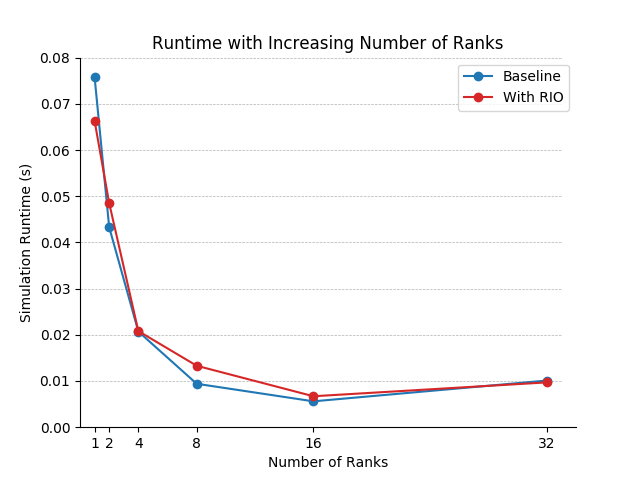
\includegraphics[scale=.6]{runtime}
	\caption{Study of runtime of simulations with 2048 LPs with varying ranks. Two data sets: runtime analysis without RIO integration and the combined checkpoint and restart simulations.} \label{fig:runtime}
\end{figure}

I used the standard modelnet-test simulation configuration with some modified variables to increase the size of the simulation. The simulations contain 2048 LPs with 2 KPs per PE. 1024 Simplenet model LPs (a model-net-base-lp derivative) and 1024 server LPs defined by the modelnet-test workload. The simulations are run for 500 nanoseconds in CODES simulation time, checkpointed, restarted, and run for an additional 500 nanoseconds.



Looking at Figure \ref{fig:runtime} we can see that RIO does not impose much overhead on simulations. The checkpoint in each case saved over a thousand in-transit events that were scheduled for after the `end' of the simulation. End in this case simply means the time of the checkpoint. The total size on disk of the checkpoint was just over 2 megabytes.


\section{A Note on Mid-Simulation Checkpointing} \label{sec:challenge}
RIO was not designed for fault-tolerance use. That is, it wasn't designed to checkpoint periodically during a running simulation to protect committed simulation history in case of failure. While theoretically, any consistent cut of the simulation would work as a checkpoint it is easier to checkpoint at a point in the simulation when all LPs are at the same point in simulation time.

There are two obvious points where all LPs are at the same point in time, the start and the end. It's simple to see how checkpointing at the start would be pointless - there'd be nothing to save. But say we wanted to run a simulation for 1000 nanoseconds. We could break this into two simulations of 500 nanoseconds each, checkpointing at the end of one and restarting at the start of the other. This would allow us to run larger simulations piecemeal, with shorter maximum runtimes than running one large run.

The way that RIO works now is that it jumps in at the end of the simulation, serializing LP state as well as all of the pending events that ROSS hadn't yet processed. At the end, there is only one location where pending events can be found. During the simulation there are more places where pending events are stored. In optimistic mode, RIO would also need to catch any in-flight events as well as anti-messages. To restart the simulation while maintaining the determinism and validity, RIO would have to ensure that the order of events processed is left unchanged between checkpoint and restart.

Additionally, mid-simulation checkpointing would require much deeper integration with ROSS. Currently RIO's checkpoint and restart behavior is performed with calls in the main method on each PE. One place where a consistent cut could be made, and RIO code could be executed, is during the all-to-all communication of GVT coordination. After all, the GVT algorithm itself is based around finding a consistent cut. Doing a RIO operation here too frequently would undoubtedly slow down the simulation if done too frequently so they should be done only every so often if mid-sim checkpointing is ever pursued.

\section{Future Work}
There was a lot of unexpected complexity in the task of serializing CODES simulations that resulted in some original milestones not being met in the three months that I worked on it. Currently RIO checkpoint/restart can be demonstrated on an optimistic simulation of CODES simplenet with a synthetic workload without sacrificing any correctness or determinism of the final state. There is not yet a serializer for other modelnet models like Fat-tree or Dragonfly and replaying traces have not yet been performed.

Next steps would be to solidify the CODES specific RIO API. After the interface is more set in stone, then a developer can implement it on larger, more complicated, network models and ensure that replaying traces does not interfere with checkpointing.


\end{document}
